\documentclass[12pt]{beamer}
\usepackage[spanish]{babel}
\usepackage[utf8]{inputenc}
\usepackage{xcolor}
\usepackage{listings}
\usepackage{textcomp}
\usepackage{mathpazo}
\usepackage{courier}
\usepackage{fancyvrb}
\usepackage{amsmath}
\usepackage{url}
\usepackage{hyperref}

\newcommand{\onelinerule}{\rule[2.3ex]{0pt}{0pt}}
\newcommand{\twolinerule}{\rule[6.2ex]{0pt}{0pt}}
\newcommand{\respuesta}{\framebox[\textwidth]{\twolinerule}}
\newcommand{\nombre}{%
  \begin{tikzpicture}[xscale=.4,yscale=.7]
    \draw (0, 0) rectangle (22, 1);
  \end{tikzpicture}%
}
%\newcommand{\rol}   {\framebox[0.3\textwidth]{\onelinerule}}
\newcommand{\rol}{%
  \begin{tikzpicture}[xscale=.4,yscale=.7]
    \draw[gray!40] ( 0, 0) grid      ( 9, 1);
    \draw          ( 0, 0) rectangle ( 9, 1);
    \draw          (10, 0) rectangle (11, 1);
    \draw (9 + .2, .5) -- (10 - .2, .5);
  \end{tikzpicture}%
}
\newcommand{\li}{\lstinline}
\providecommand{\pond}[1]{[{\small\textbf{#1\%}}]}

\lstdefinelanguage{py}{%
  classoffset=0,%
    morekeywords={%
      False,class,finally,is,return,None,continue,for,lambda,try,%
      True,def,from,nonlocal,while,and,del,global,not,with,print,%
      as,elif,if,or,yield,assert,else,import,pass,break,except,in,raise},%
    keywordstyle=\color{black!80}\bfseries,%
  classoffset=1,
    morekeywords={int,float,str,abs,len,raw_input,exit,range,min,max,%
      set,dict,tuple,list,bool,complex,round,sum,all,any,zip,map,filter,%
      sorted,reversed,dir,file,frozenset,open,%
      array,zeros,ones,arange,linspace,eye,diag,dot},
    keywordstyle=\color{black!50}\bfseries,%
  classoffset=0,%
  sensitive=true,%
  morecomment=[l]\#,%
  morestring=[b]',%
  morestring=[b]",%
  stringstyle=\em,%
}

\lstdefinelanguage{testcase}{%
  moredelim=[is][\bfseries]{`}{`},%
  backgroundcolor=\color{gray!20},%
}

\lstdefinelanguage{file}{%
  frame=single,%
}

\lstset{language=py}
\lstset{basicstyle=\ttfamily}
\lstset{columns=fixed}
\lstset{upquote=true}
\lstset{showstringspaces=false}
\lstset{rangeprefix=\#\ }
\lstset{includerangemarker=false}

\newlist{certamen}{enumerate}{1}
\setlist[certamen]{%
  label=\arabic*.,
  font=\LARGE\bfseries,%
  labelindent=-.5in,%
  leftmargin=0pt,%
  labelsep=1em%
}



\usecolortheme{seahorse}
\usefonttheme{serif}

\title{Interfaces gráficas}
\author{Programación \\ \url{http://progra.usm.cl}}
\date{}

\begin{document}
  \begin{frame}
    \maketitle
  \end{frame}

  \begin{frame}
    \label{crear-ventana}
    \frametitle{Crear una ventana}
    \begin{columns}[B]
      \column{0.6\textwidth}
        \LARGE
        \lstinputlisting{programas/tkinter/01-ventana.py}
        \vspace{10ex}
      \column{0.3\textwidth}
        \vspace{10ex}
        
\includegraphics[width=\textwidth]{programas/tkinter/capturas/01.png}
    \end{columns}
  \end{frame}

  \begin{frame}
    \label{widgets}
    \frametitle{Widgets}
    \begin{columns}
      \column{0.6\textwidth}
        \begin{itemize}
          \item \textbf{Etiqueta} (\li!Label!): \\ muestra información.
          \item \textbf{Botón} (\li!Button!):   \\ activa eventos.
          \item \textbf{Entrada} (\li!Entry!): \\ permite ingresar información.
        \end{itemize}
      \column{0.4\textwidth}
        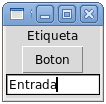
\includegraphics[width=\textwidth]{programas/tkinter/capturas/widgets.png}
    \end{columns}
  \end{frame}

  \begin{frame}
    \label{crear-widgets}
    \frametitle{Crear y agregar widgets}
    \begin{columns}[B]
      \column{0.6\textwidth}
        \footnotesize
        \lstinputlisting{programas/tkinter/04-botones.py}
      \column{0.3\textwidth}
        \vfill
        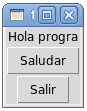
\includegraphics[width=\textwidth]{programas/tkinter/capturas/04.png}
    \end{columns}
  \end{frame}

  \begin{frame}
    \label{controladores}
    \frametitle{Controladores}
    \footnotesize
    \lstinputlisting{programas/tkinter/05-controladores.py}
  \end{frame}

  \begin{frame}
    \label{modelos}
    \frametitle{Modelos}
    \begin{columns}[B]
      \column{0.6\textwidth}
        \footnotesize
        \lstinputlisting{programas/tk-modelos.py}
      \column{0.3\textwidth}
        \vspace{20ex}
        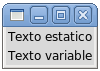
\includegraphics[width=\textwidth]{programas/tkinter/capturas/modelo.png}
    \end{columns}
  \end{frame}

  \begin{frame}
    \label{ejercicio-mas-uno}
    \frametitle{Ejercicio 1}
    Escriba un programa con la siguiente interfaz. \\
    Cada vez que se haga clic en el botón \fbox{+1}, \\
    el número mostrado debe aumentar:
    \vfill

    \begin{columns}
      \column{0.20\textwidth}
        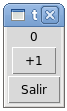
\includegraphics[width=\textwidth]{programas/tkinter/capturas/06-0.png}
      \column{0.05\textwidth}
        \(\longrightarrow\)
      \column{0.20\textwidth}
        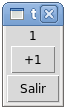
\includegraphics[width=\textwidth]{programas/tkinter/capturas/06-1.png}
      \column{0.05\textwidth}
        \(\longrightarrow\)
      \column{0.20\textwidth}
        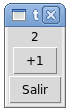
\includegraphics[width=\textwidth]{programas/tkinter/capturas/06-2.png}
      \column{0.05\textwidth}
        \(\longrightarrow\)
      \column{0.20\textwidth}
        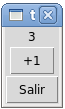
\includegraphics[width=\textwidth]{programas/tkinter/capturas/06-3.png}
    \end{columns}

   \vfill
    Al hacer clic en el botón \fbox{Salir}, \\
    el programa debe terminar.
  \end{frame}

  \begin{frame}
    \label{entrada}
    \frametitle{Entrada de datos}
    \begin{columns}[B]
      \column{0.6\textwidth}
        \footnotesize
        \lstinputlisting{programas/tk-entrada.py}
      \column{0.3\textwidth}
        \vspace{20ex}
        
\includegraphics[width=\textwidth]{programas/tkinter/capturas/entrada.png}
    \end{columns}
  \end{frame}

  \begin{frame}
    \label{resumen-conceptos}
    \frametitle{Conceptos}
    \begin{itemize}
      \Large
      \item \textbf{Controlador:} \\
        función que es invocada \\
        cuando se hace clic en un botón.
      \item \textbf{Modelo:} \\
        información que puede cambiar \\
        durante la ejecución del programa.
    \end{itemize}
  \end{frame}

  \begin{frame}
    \label{ejercicio-transformar-texto}
    \frametitle{Ejercicio 2}
    Escriba un programa con la siguiente interfaz: \\
    \vfill

    \begin{columns}
      \column{0.40\textwidth}
        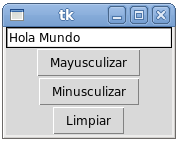
\includegraphics[width=\textwidth]{programas/tkinter/capturas/07-0.png}
      \column{0.05\textwidth}
        \(\longrightarrow\)
      \column{0.40\textwidth}
        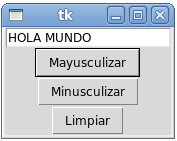
\includegraphics[width=\textwidth]{programas/tkinter/capturas/07-1.png}
    \end{columns}

   \vfill
   \fbox{Mayusculizar} debe convertir el texto a mayúsculas. \\
   \fbox{Minusculizar} debe convertir el texto a minúsculas. \\
   \fbox{Limpiar} debe borrar el texto.
  \end{frame}

  \begin{frame}
    \label{ejercicio-temperatura}
    \frametitle{Ejercicio 3}
    Escriba un programa que convierta  \\
    grados Fahrenheit a Celsius:
    \vfill

    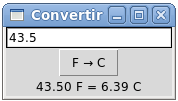
\includegraphics[width=.5\textwidth]{programas/tkinter/capturas/08.png}
    \vfill

    La fórmula es:
    \(
      \displaystyle
      C = \frac{5}{9}\cdot(F - 32)
    \)
  \end{frame}

  \begin{frame}
    \frametitle{Ejercicio 4}
    \label{ejercicio-estadisticos}
    Escriba un programa como el siguiente:
    \vfill

    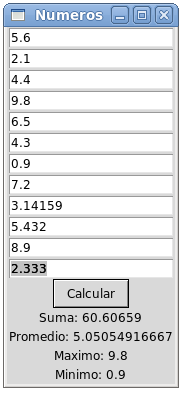
\includegraphics[width=.3\textwidth]{programas/tkinter/capturas/09.png}

  \end{frame}
\end{document}

